\documentclass[12pt,a4paper]{article}

% Formato das citações: numerica | descritiva  (mesmo estilo do modelo do TCC)
\usepackage[descritiva]{tccstyle}

% Espaçamento: o modelo do TCC usa 1,5 (ABNT). O PDF da disciplina limita o
% relatório a 5--8 páginas, então o corpo usa espaçamento simples.
% Para voltar ao 1,5, apague a linha abaixo.
\singlespacing

\usepackage{float}
\newcommand{\pend}[1]{\textcolor{red}{[\textbf{CONFIRMAR:} #1]}}

% ----------------------- METADADOS -----------------------
\titulo{ClearCut-MOG2}
\subtitulo{removedor de fundo em tempo real com subtração de fundo, sem redes neurais}
% Nomes do grupo: um por linha, separados por \\
\autor{Ruan Pedro Tirabassi\\Nome do Integrante 2\\Nome do Integrante 3}
\instituicao{Universidade Estadual do Norte do Paraná}
\campus{Luiz Meneghel}
\centro{Centro de Ciências Tecnológicas}
\curso{Bacharelado em Ciência da Computação}
\local{Bandeirantes}
\ano{2026}
\logo{logo_uenp.png}            % arquivo em figuras/
\natureza{Relatório do projeto da Avaliação 2 da disciplina de Visão
Computacional, do curso de Bacharelado em Ciência da Computação da
Universidade Estadual do Norte do Paraná.}

% Relatório de disciplina: só capa e folha de rosto (sem folha de aprovação).
\makeatletter
\renewcommand{\tcc@rosto}{%
  \begin{titlepage}\singlespacing\centering
    {\tcc@autor\par}\vspace{5cm}
    {\tcc@titcompleto\par}\vspace{2cm}
    \begin{flushright}\begin{minipage}{0.5\textwidth}\small\singlespacing
      \tcc@natureza\par\vspace{0.4cm}
      Professor: Tafarel Rocha da Silva
    \end{minipage}\end{flushright}\vfill
    {\bfseries\MakeUppercase{\tcc@local}\par\vspace{0.4cm}\tcc@ano\par}
  \end{titlepage}}
\renewcommand{\maketitle}{%
  \pagenumbering{gobble}\tcc@capa\tcc@rosto
  \pagenumbering{roman}\setcounter{page}{1}\pagestyle{empty}}
\makeatother

\begin{document}

\maketitle                       % capa + folha de rosto

\clearpage \tableofcontents      % sumário
\clearpage
\pagenumbering{arabic}\pagestyle{fancy}  % numeração visível a partir da introdução

\section{Introdução}
\label{sec:introducao}

Trocar o fundo de um vídeo é comum em videochamadas e transmissões ao
vivo: esconde o ambiente e protege a privacidade de quem está na câmera.
Para isso, o programa precisa decidir, em cada quadro e em tempo real,
quais pixels são da pessoa e quais são do fundo, um problema de
segmentação.

O ClearCut \citep{clearcut} faz isso com a webcam e troca o fundo com as
teclas A e D, mas segmenta com o \textit{SelfieSegmentation} do
MediaPipe, uma rede neural, o que não é permitido neste trabalho.
Mantivemos a experiência do ClearCut (webcam, pasta de fundos, teclas
A/D) e trocamos a segmentação por técnicas clássicas, com o conceito
novo da \textbf{subtração de fundo com MOG2}
\citep{zivkovic2004,opencv_tutorial_bgsub}.

O ClearCut-MOG2 funciona com a webcam ou com vídeos. Ele aprende a cena
vazia e, quando a pessoa entra, gera a máscara dela, conta os objetos
encontrados e cola a pessoa sobre o fundo escolhido, mostrando lado a
lado o original, a máscara e o resultado. Roda na CPU de um computador
comum, sem GPU nem modelo treinado; em troca, exige câmera parada e cena
vazia no início. Para avaliá-lo, gravamos dois vídeos com iluminação
diferente e comparamos as máscaras do programa com máscaras pintadas à
mão pelo grupo.

\section{Fundamentação teórica}
\label{sec:fundamentacao}

\subsection{Conceito novo: subtração de fundo com MOG2}
\label{sec:mog2}

A subtração de fundo parte de uma ideia simples: com a câmera parada,
tudo o que difere da cena vazia é algo que entrou nela. Comparar com
uma única foto da cena vazia falha, porque nenhum pixel é constante: o
sensor tem ruído e a compressão do vídeo mexe nos valores.

O MOG (\textit{Mixture of Gaussians}) modela \textbf{cada pixel} como
uma mistura de gaussianas \citep{stauffer1999}, cada uma com uma média
$\mu$ (a cor típica), uma variância $\sigma^2$ (o quanto o pixel
costuma variar) e um peso (com que frequência aquela cor aparece).
Várias gaussianas permitem mais de um ``jeito normal'', como uma folha
que balança na frente de uma parede. O MOG2 é a versão de
\citet{zivkovic2004} e \citet{zivkovic2006}: escolhe sozinho quantas
gaussianas cada pixel precisa (até 5 no OpenCV) e detecta sombras.

Para um pixel com cor $\mathbf{x} = (B, G, R)$, o OpenCV calcula, para
as gaussianas de maior peso, a distância
\begin{equation}
D^2 = \frac{(B-\mu_B)^2 + (G-\mu_G)^2 + (R-\mu_R)^2}{\sigma^2}
\label{eq:mog2}
\end{equation}
e considera o pixel \textbf{fundo} quando $D^2 < T$, em que $T$ é o
parâmetro \texttt{varThreshold} \citep{opencv_mog2}. Dividir pela
variância é o que torna o teste justo: num pixel que varia muito, uma
diferença grande ainda é normal; numa parede lisa, uma diferença pequena
já é suspeita. O OpenCV impõe um piso de $\sigma^2 = 4$ à variância.

Se o pixel não é fundo, o MOG2 ainda testa se ele é uma
\textbf{sombra}: se a cor é a mesma do fundo, só que mais escura (entre
50\% e 100\% do brilho original), ele recebe o valor 127 em vez de 255
na saída.

Enquanto aprende, a cada quadro a gaussiana que explica a cor nova
ganha peso e tem a média puxada na direção dela, com intensidade dada
pelo \texttt{learningRate} ($-1$: o OpenCV escolhe; $0$: modelo
\textbf{congelado}). Aprendemos a cena vazia e depois congelamos, para
que uma pessoa parada não vire fundo com o tempo.

\paragraph{Exemplo feito à mão.} Considere um pixel de uma parede cinza
aprendido com $\mu = (150, 150, 150)$. Como a parede é lisa, a
variância fica no piso, $\sigma^2 = 4$. Com $T = 40$
(Tabela~\ref{tab:exemplo}):

\begin{table}[H]
\centering
\caption{Classificação de um pixel de parede ($\mu = 150$, $\sigma^2 = 4$, $T = 40$) pela Equação~\ref{eq:mog2}.}
\label{tab:exemplo}
\small
\begin{tabular}{llll}
\toprule
Cor nova $(B,G,R)$ & Conta & $D^2$ & Saída \\
\midrule
$(156, 156, 156)$ & $(6^2+6^2+6^2)/4$ & $27 < 40$ & fundo (0) \\
$(158, 158, 158)$ & $(8^2+8^2+8^2)/4$ & $48 > 40$ & frente (255) \\
$(55, 60, 45)$, camiseta & $(95^2+90^2+105^2)/4$ & $\approx 7038$ & frente (255) \\
$(120, 120, 120)$, mais escura & mesma cor, 80\% do brilho & --- & sombra (127) \\
\bottomrule
\end{tabular}
\end{table}

O exemplo mostra que, numa parede lisa, um clareamento uniforme de
apenas 8 níveis (de 0 a 255) já transforma o pixel em ``pessoa''. Em
geral, clareando $d$ níveis nos três canais, $D^2 = 3d^2/\sigma^2$, e o
pixel continua fundo enquanto $d < \sqrt{T\sigma^2/3}$, isto é,
$d < 7{,}3$ para $T = 40$ (Figura~\ref{fig:mog2}). Conferimos a conta
com uma parede sintética (cinza 150 com ruído): clareando 6 níveis,
nenhum pixel virou frente; clareando 8, 99\% viraram. Esse limite
apertado explica o maior problema que encontramos
(Seção~\ref{sec:exposicao}): quando a câmera ajusta o brilho sozinha,
a parede inteira vira ``pessoa''.

\begin{figure}[H]
\centering
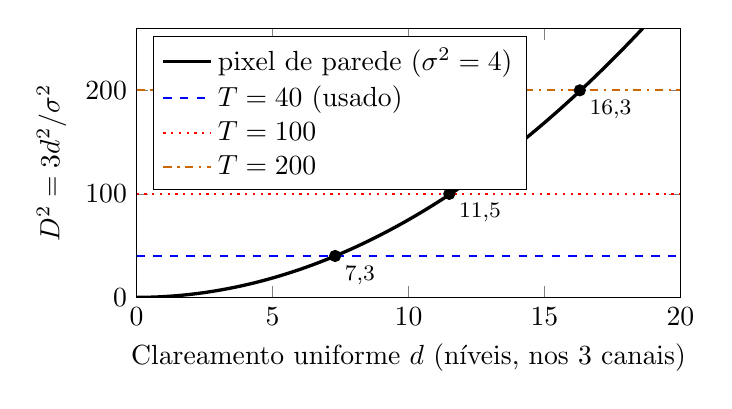
\begin{tikzpicture}
\begin{axis}[
  width=0.7\linewidth, height=5cm,
  xlabel={Clareamento uniforme $d$ (níveis, nos 3 canais)},
  ylabel={$D^2 = 3d^2/\sigma^2$},
  xmin=0, xmax=20, ymin=0, ymax=260,
  legend pos=north west, legend cell align=left]
\addplot[domain=0:20, samples=100, very thick, black] {3*x^2/4};
\addlegendentry{pixel de parede ($\sigma^2 = 4$)}
\addplot[domain=0:20, thick, dashed, blue] {40};
\addlegendentry{$T = 40$ (usado)}
\addplot[domain=0:20, thick, dotted, red] {100};
\addlegendentry{$T = 100$}
\addplot[domain=0:20, thick, dashdotted, orange!80!black] {200};
\addlegendentry{$T = 200$}
\addplot[only marks, mark=*, mark size=2pt, black] coordinates {(7.3,40) (11.5,100) (16.3,200)};
\node[anchor=north west, font=\footnotesize] at (axis cs:7.3,40) {7,3};
\node[anchor=north west, font=\footnotesize] at (axis cs:11.5,100) {11,5};
\node[anchor=north west, font=\footnotesize] at (axis cs:16.3,200) {16,3};
\end{axis}
\end{tikzpicture}
\caption{Quanto uma parede lisa pode clarear antes de virar ``pessoa'':
o pixel é fundo enquanto a curva está abaixo da linha do limiar $T$.
Figura feita pelo grupo a partir da Equação~\ref{eq:mog2}.}
\label{fig:mog2}
\end{figure}

O mesmo cálculo mostra o caso contrário, a \textbf{camuflagem}. Se a
camiseta $(55, 60, 45)$ passa na frente de um objeto escuro
$(40, 40, 40)$ cuja variância aprendida é $\sigma^2 = 25$, então
$D^2 = (15^2 + 20^2 + 5^2)/25 = 26 < 40$, e aquele pedaço da pessoa é
classificado como fundo. O MOG2 só compara cores; se a pessoa tem a cor
do que está atrás dela, ele não tem como separá-las.

\subsection{Técnicas vistas em aula}
\label{sec:tecnicas}

\textbf{Filtro gaussiano.} Substitui cada pixel por uma média ponderada
da vizinhança, com pesos maiores no centro
\citep{gonzalez2010}. Usamos um kernel $5 \times 5$ antes do MOG2 para
reduzir o ruído do sensor, que faria pixels isolados ``piscarem'' como
se fossem movimento.

\textbf{Limiarização.} Transforma uma imagem em cinza em binária: o que
está acima do limiar vira 255 e o resto vira 0 \citep{gonzalez2010}. A
saída do MOG2 tem três valores (0 fundo, 127 sombra, 255 frente);
limiarizando em 200, só a frente sobra, e a sombra que a pessoa projeta
na parede não é confundida com ela.

\textbf{Morfologia.} A erosão encolhe as regiões brancas e a dilatação
as expande, usando um elemento estruturante \citep{gonzalez2010}. A
\textbf{abertura} (erosão seguida de dilatação) apaga pontos soltos de
ruído; o \textbf{fechamento} (dilatação seguida de erosão) tapa buracos
pequenos dentro da silhueta. Usamos um elemento elíptico $7 \times 7$.

\textbf{Contornos e área.} O \texttt{findContours} encontra as bordas de
cada região branca. Descartamos as regiões com área menor que um mínimo
(manchas que a morfologia não removeu) e desenhamos as restantes
preenchidas, o que fecha buracos internos maiores. O número de regiões
que sobram é o \textbf{número de objetos}, o descritor que o programa
mostra na tela.

\textbf{Composição com borda suave.} Desfocar a máscara binária cria uma
transição de 0 a 1 na borda, o canal alfa ($\alpha$). O resultado é
$\alpha \cdot \text{quadro} + (1-\alpha) \cdot \text{fundo novo}$; sem o
desfoque, o recorte fica serrilhado.

\textbf{IoU} (\textit{Intersection over Union}). Pixels de pessoa em
comum entre duas máscaras divididos pelos pixels de pessoa em pelo
menos uma delas: 1 quando são idênticas, 0 quando não se tocam.
Preferimos o IoU à acurácia de pixels porque o fundo ocupa a maior
parte da imagem, e um programa que errasse metade da pessoa ainda teria
acurácia acima de 90\%.

\section{Metodologia}
\label{sec:metodologia}

\subsection{Dados}

Gravamos dois vídeos com o celular apoiado, no mesmo quarto:
\texttt{video\_claro} (32\,s, luz acesa) e \texttt{video\_escuro}
(30\,s, pouca luz). Os dois começam com 2 a 3 segundos de cena vazia;
depois a pessoa entra, senta, acena, levanta e chega perto da câmera,
com um ventilador preto, uma cadeira e uma cama ao fundo. A
demonstração ao vivo usa a webcam do notebook ($640 \times 480$).

\subsection{Pipeline}

A Figura~\ref{fig:pipeline} mostra o caminho de cada quadro até a
resposta. Na fase 1, os 60 primeiros quadros, com a cena vazia, treinam
o MOG2 com \texttt{learningRate} $= -1$; na fase 2, cada quadro passa
pelas etapas 0 a 7 com o modelo congelado. Na webcam, uma contagem
regressiva de 5 segundos antes da fase 1 dá tempo de a pessoa sair da
cena.

\begin{figure}[H]
\centering
\begin{tikzpicture}[node distance=5mm and 3mm,
  passo/.style={stepbox, minimum height=1.55cm}]
\node[passo] (e) {\textbf{Entrada}\\quadro da webcam ou do vídeo, altura 480};
\node[passo, right=of e] (p0) {\textbf{0. Compensação}\\ganho por cor = moda de fundo/quadro};
\node[passo, right=of p0] (p1) {\textbf{1. Filtro gaussiano}\\$5 \times 5$};
\node[passo, right=of p1, fill=orange!20] (p2) {\textbf{2. MOG2}\\aprende 60 quadros e depois congela};
\node[passo, right=of p2] (p3) {\textbf{3. Limiar 200}\\descarta a sombra (127)};
\node[passo, below=of p3] (p4) {\textbf{4. Abertura e fechamento}\\elipse $7 \times 7$};
\node[passo, left=of p4] (p5) {\textbf{5. Contornos}\\área $\geq 2000$, preenchidos; contagem};
\node[passo, left=of p5] (p6) {\textbf{6. Buracos}\\maiores que 1500\,px voltam a ser fundo};
\node[passo, left=of p6] (p7) {\textbf{7. Composição}\\erosão $5 \times 5$, desfoque $9 \times 9$, alfa};
\node[passo, left=of p7] (s) {\textbf{Saída}\\original, máscara, resultado e nº de objetos};
\draw[arrow] (e) -- (p0);
\draw[arrow] (p0) -- (p1);
\draw[arrow] (p1) -- (p2);
\draw[arrow] (p2) -- (p3);
\draw[arrow] (p3) -- (p4);
\draw[arrow] (p4) -- (p5);
\draw[arrow] (p5) -- (p6);
\draw[arrow] (p6) -- (p7);
\draw[arrow] (p7) -- (s);
\end{tikzpicture}
\caption{Pipeline do ClearCut-MOG2. Em laranja, o conceito novo.}
\label{fig:pipeline}
\end{figure}

As etapas 1, 3, 4 e 5 são as técnicas da Seção~\ref{sec:tecnicas}. A
etapa 6 existe porque o preenchimento da etapa 5 tapa \textbf{todos} os
buracos, inclusive o vão entre o braço e o corpo com a mão na cintura,
onde reaparecia a parede antiga. Na etapa 7, a máscara é encolhida
antes do desfoque, para não deixar um halo da parede antiga em volta da
pessoa.

\subsection{Parâmetros}

Os parâmetros são constantes comentadas no topo do código
(Tabela~\ref{tab:parametros}). O processamento leva de 27 a 30\,ms por
quadro na webcam, cerca de 35 quadros por segundo, acima dos 30 que ela
entrega.

\begin{table}[H]
\centering
\caption{Parâmetros do pipeline e como foram escolhidos.}
\label{tab:parametros}
\small\setstretch{1.0}
\begin{tabularx}{\linewidth}{>{\raggedright\arraybackslash}p{3.6cm} l >{\raggedright\arraybackslash}X}
\toprule
Constante (etapa) & Valor & Como chegamos \\
\midrule
\texttt{BLUR} (1) & 5 & Valor usado em aula; não variamos. \\
\texttt{FRAMES\_APRENDER} (2) & 60 & Cerca de 2\,s; cabe no início vazio dos vídeos. \\
\texttt{VAR\_THRESHOLD} (2) & 40 & Testamos de 10 a 200. Acima de 40 aumentam os buracos; abaixo, os vídeos melhoram, mas surgem manchas falsas na webcam (Seção~\ref{sec:discussao}). \\
\texttt{LIMIAR} (3) & 200 & Qualquer valor entre 128 e 254 separa sombra (127) de frente (255). \\
\texttt{KERNEL} (4) & 7 & Com 11, o IoU médio caiu de 0,791 para 0,764: a silhueta engorda e perde dedos. \\
\texttt{AREA\_MIN} (5) & 2000 & Maior que as manchas de ruído observadas; não variamos. \\
\texttt{BURACO\_MAX} (6) & 1500 & Na webcam, os vãos entre braço e corpo mediram 2345 e 3104\,px; as falhas de detecção, no máximo 1071\,px. \\
\texttt{ENCOLHER\_BORDA}, \texttt{SUAVIZAR\_BORDA} (7) & 5 e 9 & Comparação visual: sem erosão e com desfoque 15, aparecia um halo claro em volta da pessoa. \\
\texttt{ESPERA\_WEBCAM} & 5\,s & Tempo para sair da cena e para a webcam estabilizar o brilho. \\
\bottomrule
\end{tabularx}
\end{table}

\subsection{Exposição automática: compensação e trava}
\label{sec:exposicao}

O maior problema do projeto veio da câmera, não do MOG2. Quando a
pessoa de camiseta escura entra, a câmera aumenta a exposição sozinha.
Numa gravação de teste, a parede clareou 22 níveis (de 152 para 174),
muito além dos 7,3 que ela tolera (Figura~\ref{fig:mog2}); no vídeo
claro, 92\% da imagem foi marcada como pessoa
(Figura~\ref{fig:exposicao}b).

\textbf{Compensação (etapa 0).} Multiplicamos cada canal do quadro por
um ganho que o devolve ao brilho do fundo aprendido. O ganho é o valor
\textbf{mais comum} (a moda do histograma) da razão fundo
aprendido / quadro: quando a câmera clareia, todos os pixels do fundo
pedem o mesmo ganho e formam um pico, enquanto os da pessoa ficam
espalhados; por isso funciona mesmo com a pessoa ocupando mais da
metade da imagem (Figura~\ref{fig:exposicao}c). Foi a terceira versão:
a mediana da imagem inteira era puxada pela pessoa, e a mediana só do
fundo do quadro anterior chegava a inverter a máscara.

\textbf{Trava (webcam).} Na webcam, com a pessoa perto, a parede foi de
130 para 235, e de 19\% a 31\% dos pixels estouraram em 255. A câmera
também muda a curva de tons: no mesmo quadro, a parte clara da parede
pedia ganho 0,70 e a escura, 0,59, e nenhum ganho único corrige as duas
(Figura~\ref{fig:exposicao}d--e). Por isso, depois da contagem, o
programa \textbf{trava} a exposição pelo OpenCV
(\texttt{CAP\_PROP\_AUTO\_EXPOSURE}), testando cinco valores e ficando
com o de brilho mais próximo do automático. Ao reaprender o fundo
(tecla B) ou sair, a câmera volta ao automático. Com a trava, a parede
ficou entre 108 e 118 o teste inteiro (Figura~\ref{fig:exposicao}f--g).

\begin{figure}[H]
\centering
\includegraphics[width=\linewidth]{fig_exposicao.jpg}
\caption{Exposição automática. Vídeo claro: (a) quadro, (b) máscara sem
compensação e (c) com compensação. Webcam: (d--e) sem a trava, o fundo
some; (f--g) com a trava, a máscara mostra só a pessoa.}
\label{fig:exposicao}
\end{figure}

\subsection{Avaliação}

Escolhemos 12 quadros, 6 de cada vídeo, todos com a pessoa e misturando
casos fáceis e difíceis. Quadros vazios ficaram de fora, porque programa
e gabarito vazios dão IoU $= 1$ e inflariam o resultado. Para cada
quadro, o grupo pintou à mão a máscara correta (gabarito) com uma
ferramenta própria (\texttt{criar\_gabarito.py}), e o
\texttt{avaliacao.py} calcula o IoU e conta \textbf{acerto} quando
IoU $\geq 0{,}8$. Também conferimos a contagem de objetos nos 78 quadros
salvos (1 a cada 20). Como o sistema não classifica objetos em classes,
não há matriz de confusão.

\section{Resultados}
\label{sec:resultados}

A Figura~\ref{fig:antesdepois} mostra o antes e o depois nos dois vídeos
e na webcam. No painel da webcam aparece o texto que o programa escreve
na tela: o fundo atual e o número de objetos.

\begin{figure}[H]
\centering
\includegraphics[width=0.9\linewidth]{fig_antes_depois.jpg}
\caption{Antes e depois. Em cada grupo, da esquerda para a direita:
quadro original, máscara e resultado. (a) Vídeo claro, quadro 520; (b)
vídeo escuro, quadro 580, com o braço separado do corpo contado como
segundo objeto; (c) webcam, na demonstração gravada.}
\label{fig:antesdepois}
\end{figure}

A Tabela~\ref{tab:acertos} traz o resultado da avaliação nos 12 quadros
com gabarito.

\begin{table}[H]
\centering
\caption{IoU entre a máscara do programa e o gabarito pintado à mão.
Acerto quando IoU $\geq 0{,}8$.}
\label{tab:acertos}
\small\setstretch{1.1}
\begin{tabular}{llllc}
\toprule
Vídeo & Quadro & Situação & IoU & Resultado \\
\midrule
Claro  & 520 & entrando, em pé                  & 0,844 & acerto \\
Claro  & 600 & sentado, ventilador atrás         & 0,751 & erro \\
Claro  & 760 & acenando, ventilador atrás        & 0,753 & erro \\
Claro  & 820 & braço levantado                   & 0,787 & erro \\
Claro  & 880 & em pé, ventilador atrás           & 0,772 & erro \\
Claro  & 940 & bem perto da câmera               & 0,829 & acerto \\
\midrule
Escuro & 400 & entrando, borrado de movimento    & 0,748 & erro \\
Escuro & 460 & sentado                           & 0,783 & erro \\
Escuro & 540 & acenando                          & 0,741 & erro \\
Escuro & 580 & braço levantado                   & 0,816 & acerto \\
Escuro & 680 & em pé, perto                      & 0,791 & erro \\
Escuro & 720 & bem perto da câmera               & 0,875 & acerto \\
\midrule
\multicolumn{3}{l}{\textbf{Total: 4 acertos em 12 (33,3\%)}} & \textbf{0,791} & (média) \\
\bottomrule
\end{tabular}
\end{table}

O sistema acertou 2 dos 6 quadros em cada vídeo, \textbf{4 de 12 no
total (33,3\%)}, com IoU médio de \textbf{0,791}. A taxa baixa esconde
um resultado mais equilibrado: nenhum quadro ficou abaixo de 0,74, e
três erros ficaram entre 0,78 e 0,80, logo abaixo do critério.

O erro é quase todo de um tipo só (Figura~\ref{fig:avaliacao}): o
programa deixou de fora de 12\% a 26\% da pessoa em cada quadro, mas
quase nunca marcou fundo como pessoa (no máximo 2,6\% a mais). As
falhas se concentram na camiseta escura na frente do ventilador preto e
no short na frente da cadeira, a camuflagem prevista na
Seção~\ref{sec:mog2}.

\begin{figure}[H]
\centering
\includegraphics[width=0.75\linewidth]{fig_avaliacao.jpg}
\caption{Máscara do programa comparada com o gabarito. Verde: acerto;
vermelho: pessoa que o programa deixou de fora; azul: fundo marcado
como pessoa. Nos quadros claro 600 e 820, o buraco redondo é a camiseta
na frente do ventilador.}
\label{fig:avaliacao}
\end{figure}

A contagem de objetos acertou em \textbf{75 dos 78 quadros salvos
(96,2\%)}. Nos 36 quadros sem ninguém, ela deu 0; nos 42 com a pessoa,
deu 1 em 39. Os três erros (claro 820 e escuro 580 e 660) contaram 2
objetos, porque o braço levantado se separou do corpo na máscara.

\section{Discussão}
\label{sec:discussao}

\textbf{Camuflagem.} É o principal erro que sobrou. Onde a camiseta
escura passa na frente do ventilador preto, ou o short na frente da
cadeira, as cores ficam a uma distância $D^2$ menor que o limiar, e o
MOG2 classifica aquele pedaço da pessoa como fundo
(Seção~\ref{sec:mog2}). Como o método só compara cores, nenhum
parâmetro resolve isso sem criar outro erro. Uma melhoria seria usar
também textura ou bordas, que mudam quando a pessoa entra mesmo com cor
parecida. Na demonstração, a solução prática é tirar objetos escuros de
trás da pessoa.

\textbf{Todo ajuste é uma troca.} Com o \texttt{varThreshold} em 16, o
MOG2 fica mais sensível e tapa parte da camuflagem: os acertos nos
vídeos subiram de 4 para 8 (IoU médio 0,821). Na gravação da webcam,
porém, os quadros com mais de um objeto passaram de 14 para 128, em
603: a pessoa perto da câmera muda levemente a luz da cama ao lado
(sombra e reflexo), e com o limiar baixo isso já vira mancha. Da mesma
forma, sem a etapa 6 os acertos subiriam de 4 para 6, porque um buraco
de camuflagem dentro da silhueta é igual, para o programa, ao vão entre
o braço e o corpo; mas a parede antiga voltaria a aparecer nesse vão.
Mantivemos os valores testados ao vivo. Escolher o limiar olhando os
mesmos 12 quadros da avaliação, aliás, deixaria o número otimista.

\textbf{Contagem.} Os três erros de contagem foram o braço levantado
separado do corpo, quase sempre porque a camiseta entre eles sumiu por
camuflagem. Juntar contornos próximos resolveria esses casos, mas
juntaria também duas pessoas lado a lado.

\textbf{O gabarito também erra.} Na primeira avaliação, o IoU médio foi
0,769. A sobreposição mostrou que o gabarito passava de 4 a 8\,px para
fora da pessoa: a ferramenta mostrava o quadro pequeno (269\,px de
largura) e o pincel era grande. Com zoom e um modo de correção na
ferramenta, o grupo corrigiu as bordas, e o IoU médio foi para 0,791,
sem nenhuma mudança no programa.

\textbf{Mudança de luz.} Congelar o modelo faz uma pessoa parada
continuar aparecendo, mas impede o MOG2 de se adaptar se a luz do
ambiente mudar. Uma melhoria seria atualizar o modelo devagar, só fora
da máscara da pessoa; hoje, a tecla B reaprende o fundo. Pelo mesmo
motivo, a cena precisa estar vazia no aprendizado: nos primeiros testes
com a webcam, a pessoa ficou na frente da câmera, virou parte do fundo
e só os contornos dela apareciam, o que motivou a contagem regressiva.

\section{Conclusão}
\label{sec:conclusao}

Construímos um removedor de fundo em tempo real para webcam e vídeos,
sem redes neurais, combinando a subtração de fundo com MOG2 e as
técnicas vistas em aula. O MOG2 decide, pixel a pixel, o que é pessoa,
e as outras etapas limpam e completam essa decisão. O sistema acertou a
contagem de objetos em 96,2\% dos quadros e chegou a um IoU médio de
0,791, com 4 de 12 quadros acima do critério de 0,8.

A principal lição foi que quase todos os erros vieram de quebrar um
pressuposto do método, e não do algoritmo: a câmera que muda a
exposição sozinha, a pessoa na cena durante o aprendizado e a roupa da
cor do fundo. O exemplo feito à mão mostrou por que a exposição era tão
grave e por que aumentar o limiar não resolvia. Aprendemos também a
medir antes de mudar: medir o brilho da parede revelou a causa, e a
melhor correção para a webcam foi na captura, travando a exposição.
Por fim, vimos que todo ajuste é uma troca e que até o gabarito precisa
ser conferido antes de se confiar no número.

\section{Uso de ferramentas de inteligência artificial}
\label{sec:ia}

Usamos o Claude (Anthropic), pelo Claude Code no VS Code, como apoio
durante todo o projeto:

\begin{itemize}[nosep]
  \item \textbf{Código:} escrever a primeira versão dos programas a
  partir da especificação que o grupo preparou (pipeline, constantes
  comentadas, ferramenta de gabarito e script de avaliação).
  \item \textbf{Testes e diagnóstico:} gerar vídeos sintéticos para
  testar o código e analisar os nossos vídeos e gravações da webcam.
  Exemplos: identificar a exposição automática como causa do fundo que
  sumia e a borda larga dos gabaritos.
  \item \textbf{Correções:} propor e testar a contagem regressiva, as
  versões da compensação de exposição, a trava da webcam e os ajustes
  de borda.
  \item \textbf{Relatório:} organizar as anotações de cada teste, gerar
  as figuras a partir dos nossos resultados e redigir um rascunho deste
  texto, que o grupo revisou.
\end{itemize}

As gravações, os testes com a webcam, a pintura dos gabaritos, a escolha
dos casos difíceis e as decisões sobre o que manter foram feitos pelo
grupo, que revisou o código e o texto e é responsável por explicá-los.


\clearpage
\phantomsection
\addcontentsline{toc}{section}{REFERÊNCIAS}
\bibliographystyle{\tccbibstyle}
\bibliography{referencias}

\end{document}
